%
% 2-geodaeten.tex
%
% (c) 2025 Prof Dr Andreas Müller
%

%
% Geodäten
%
\section{Geodäten
\label{buch:zusammenhang:section:geodaeten}}
\kopfrechts{Geodäten}
Die kovariante Ableitung war motiviert als ein Kriterium, mit
dem man erkennen kann, ob ein Vektor parallel transportiert
worden ist.
Eine Geodäte kann daher als Kurve definiert werden, entlang der
der Tangentialvektor parallel transportiert wird.
Diese Bedingung äussert sich als Differentialgleichung, die in
Abschnitt~\ref{buch:zusammenhang:geodaeten:subsection:differentiagleichung}
diskutiert wird.
Meist werden Geodäten aber Kurven minimaler Länge zwischen zwei Punkten
definiert.
Sie minimieren das Längenfunktional, welches aus der Metrik gewonnen
werden kann.
Nach den Regeln der Variationsrechnung lässt sich aus dem Längenfunktional
mit der Euler-Lagrange-Differentialgleichung eine Differentialgleichung
für die kürzesten Kurven finden.
In Abschnitt~\ref{buch:zusammenhang:geodaeten:subsection:kuerzeste}
wird gezeigt, dass sie mit der Differentialgleichung übereinstimmt.

%
% Differentialgleichung
%
\subsection{Differentialgleichung für Geodäten
\label{buch:zusammenhang:geodaeten:subsection:differentialgleichung}}
Eine Geodäte ist eine Kurve, entlang der der Tangentialvektor an die
Kurve parallel transportiert wird.
Dies bedeutet, dass in jedem Punkt der Kurve $\gamma(t)$ die kovariante
Ableitung des Tangentialvektors $\dot{\gamma}$ in Richtung
$\dot{\gamma}$ verschwindet.
Es gilt also
\[
\nabla_{\dot{\gamma}(t)} \dot{\gamma}(t)
=
0
\]
Die Komponenten des Tangentialvektors in einer Karte sind $\dot{x}^i(t)$.
Mit den Christoffel-Symbolen ist die kovariante Ableitung
\begin{align*}
\dot{x}^k
\biggl(
\frac{\partial\dot{x}^i}{\partial x^k}
+
\Gamma^i_{kl}\dot{x}^l
\biggr)
&=
0
\\
\frac{\partial\dot{x}^i}{\partial x^k}
\dot{x}^k
+
\Gamma^i_{kl} \dot{x}^l \dot{x}^k
&=
0.
\end{align*}
Der erste Term ist wegen
\[
\frac{dA^i}{dt}
=
\frac{\partial A^i}{\partial x^k}\frac{dx^k}{dt}
=
\frac{\partial A^i}{\partial x^k}
\dot{x}^k
\]
die Ableitung von $\dot{x}^i$ nach der Zeit.

\begin{satz}
Eine Geodäte $\gamma(t)$ erfüllt in jeder Karte die Differentialgleichung
\begin{equation}
\ddot{x}^i
+
\Gamma^i_{kl} \dot{x}^l \dot{x}^k
=
0.
\label{buch:zusammenhang:geodaeten:eqn:dgl}
\end{equation}
\end{satz}

%
% Beispiele
%
\subsection{Beispiele
\label{buch:zusammenhang:geodaeten:subsection:beispiele}}
Falls die Christoffel-Symbole alle verschwinden, bleibt von der
Differentialgleichung~\eqref{buch:zusammenhang:geodaeten:eqn:dgl}
nur noch die Gleichungen
\[
\ddot{x}^i = 0
\]
übrig, welche als Lösungen alle Geraden im $n$-dimensionalen
Raum haben.

%
% Polarkoordinaten
%
\subsubsection{Polarkoordinaten}
Für Polarkoordinaten wurden die Christoffel-Symbole bereits
in Beispiel~\ref{buch:zusammenhang:paralleltransport:bsp:polar}
berechnet.
Die Differentialgleichungen
\begin{align*}
\ddot{x}^i=-\Gamma^i_{kl}\dot{x}^k\dot{x}^l
\end{align*}
können mit den Resultaten von 
Beispiel~\ref{buch:zusammenhang:paralleltransport:bsp:polar}
ausgeschrieben werden als die beiden Differentialgleichungen
\begin{equation}
\left.
\begin{aligned}
\ddot{x}^1
&=
\Gamma^1_{22}(\dot{x}^2)^2
\\
\ddot{x}^2
&=
\Gamma^2_{21}\dot{x}^1\dot{x}^2
+
\Gamma^2_{12}\dot{x}^2\dot{x}^1
\end{aligned}
\quad
\right\}
\qquad
\Rightarrow
\qquad
\left\{
\quad
\begin{aligned}
\ddot{r}
&=
r \dot{\varphi}^2
\\
\ddot{\varphi}
&=
-\frac{2}{r}\dot{\varphi}\dot{r}
\end{aligned}
\right.
\label{buch:zusammenhang:paralleltransport:bsp:polardgl}
\end{equation}
Daraus lässt sich bereits ablesen, dass die radialen Geraden, die
durch $\varphi=\text{const}$ charakterisiert sind, Lösungen
der Differentialgleichung
\eqref{buch:zusammenhang:paralleltransport:bsp:polardgl}
sind.
In diesem Fall ist $\ddot{\varphi}=\dot{\varphi}=0$ und
daher $\ddot{r}=0$, die als Lösung $r=vt+r_0$, wobei $v$ die Geschwindigkeit
und $r_0$ der Radius zur Zeit $t=0$ ist.

Schreibt man $\omega=\dot{\varphi}$ für die Winkelgeschwindigkeit, dann
wird die zweite Gleichung von
\eqref{buch:zusammenhang:paralleltransport:bsp:polardgl}
zu
\[
\frac{\dot{\omega}}{\omega}
=
-2\frac{\dot{r}}{r}
\qquad\Rightarrow\qquad
\frac{d}{dt}\log \omega
=
\frac{d}{dt}\bigl(-2\log r\bigr)
=
\frac{d}{dt}\log\frac{1}{r^2}.
\]
Durch Integration findet man, dass
\begin{equation}
\log \omega = \log\frac{1}{r^2} + C
\qquad\Rightarrow\qquad
\omega = \frac{D}{r^2}
\qquad\Rightarrow\qquad
\omega r^2 = D
\label{buch:zusammenhang:paralleltransport:bsp:drehimpuls}
\end{equation}
mit $D=e^C$ ist.
Multipliziert man die letzte Gleichung mit $m$, erhält man
$m\omega r^2=\text{const}$, also die Aussage, dass der Drehimpuls
erhalten ist.
Jeder Massepunkt, der sich in der Ebene mit konstanter Geschwindigkeit
und konstanter Richtung bewegt, erfüllt diese Gleichung.

Mit der Drehimpulserhaltung
\eqref{buch:zusammenhang:paralleltransport:bsp:drehimpuls}
kann jetzt 
die zweite Differentialgleichung von
\eqref{buch:zusammenhang:paralleltransport:bsp:polardgl}
zu
\begin{equation}
\ddot{r}=r\biggl(\frac{D}{r^2}\biggr)^2 = r^{-3} D^2
\label{buch:zusammenhang:paralleltransport:bsp:polardotr}
\end{equation}
vereinfacht werden.
Schreibt man $r=\sqrt{R}$ oder $r^2=R$, werden die Ableitungen von $R$
\begin{align*}
\dot{R} &= 2\dot{r} r \\
\ddot{R}
&=
2\ddot{r} r + 2\dot{r}^2
=
\\
\dddot{R}
&=
2\dddot{r} r + 2\ddot{r}\dot{r} + 4\ddot{r}\dot{r}
=
2\dddot{r}r + 6\ddot{r}\dot{r}
\intertext{oder nach Einsetzen von 
\eqref{buch:zusammenhang:paralleltransport:bsp:polardotr}
und dessen Ableitung
}
&=
2(-3\dot{r}r^{-4}D^2) r + 6r^{-3}D^2\dot{r}
=
6\dot{r}D^2(-r^{-3}+r^{-3})
=
0.
\end{align*}
Es folgt, dass $R$ ein quadratisches Polynom in $t$ sein muss.
Es muss von der Form $R=at^2 + bt + c$ sein.
Da $R(t)\ge 0$ sein muss, muss $a \ge 0$ sein und die Diskriminante $\Delta$
muss 
\[
\Delta
=
b^2-4ac\le 0
\]
sein.
Für $a>0$ kann man dies durch quadratisches Ergänzen in die Form
\[
R(t)
=
a\biggl(t+\frac{b}{2a}\biggr)^2 - \frac{b^2-4ac}{4a^2}
\]
bringen.
Das Minimum wird erreicht wenn $t=-b/2a$ ist, daher kann man die
Parameter wie folgt interpretieren.
%
% fig-polargeodaete.tex
%
% (c) 2025 Prof Dr Andreas Müller
%
\begin{figure}
\centering
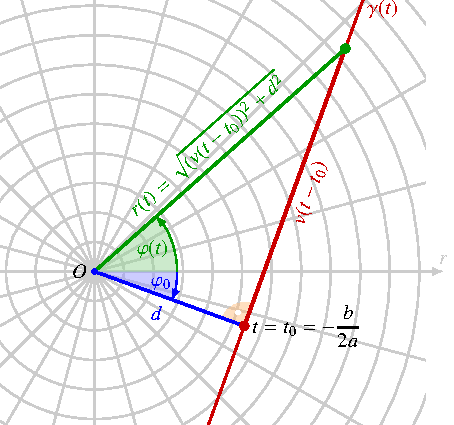
\includegraphics{chapters/100-zusammenhang/images/polargeodaete.pdf}
\caption{Geodäten in Polarkoordinaten sind Geraden.
Der Radius in Abhängigkeit vom Parameter ist $r(t)$, die Gerade
geht für den Parameterwert $t_0=-b/2a$ im kleinsten Abstand $d$
am Nullpunkt vorbei.
\label{buch:zusammenhang:geodaeten:fig:polargeodaete}}
\end{figure}
%
Schreibt man
\[
t_0=-b/2a,
\qquad
v=\sqrt{a}
\qquad\text{und}\qquad
d^2 = -\frac{b^2-4ac}{4a^2},
\]
folgt
\[
R(t)
=
(v(t-t_0))^2 + d^2
\qquad\Rightarrow\qquad
r(t)
=
\sqrt{
(v(t-t_0))^2 + d^2
}.
\]
Daraus kann man mit Hilfe des Satzes von Pythagoras ablesen, dass sich
der Punkt mit der Geschwindigkeit $v$ auf einer Geraden bewegt und
zur Zeit $t_0$ im geringsten Abstand $d$ am Nullpunkt vorbeigeht
(Abbildung~\ref{buch:zusammenhang:geodaeten:fig:polargeodaete}).
Damit lässt sich jetzt auch die Konstante $D$ bestimmen.
Aus $v=\omega d$ folgt
\[
\omega=\frac{d}{v}
\quad \Rightarrow \quad
D=\omega d^2 = \frac{d^3}{v}
\]

Aus $\dot{\varphi}=\omega = Dr^{-2} = d^3 / v r^2$
kann jetzt durch Integration auch die explizite Formel 
\[
\varphi(t)
=
\varphi_0
+
\frac{d}{v}
\int_{t_0}^t
\frac{d^2\,dt}{v^2(t-t_0)^2+d^2}
=
\varphi_0
+
\frac{d}{v}
\arctan\frac{(t-t_0)v}{d}
\]
für $\varphi(t)$ gefunden werden.

%
% Geodäten auf einer Kugeloberfläche
%
\subsubsection{Geodäten auf einer Kugeloberfläche}
In Beispiel~\ref{buch:zusammenhang:paralleltransport:bsp:kugel}
wurden die Christoffel-Symbole für Kugelkoordinaten auf einer
Kugeloberfläche berechnet.
%
% kugeldreieck.tex
%
% (c) 2025 Prof Dr Andreas Müller
%
\begin{figure}
\centering
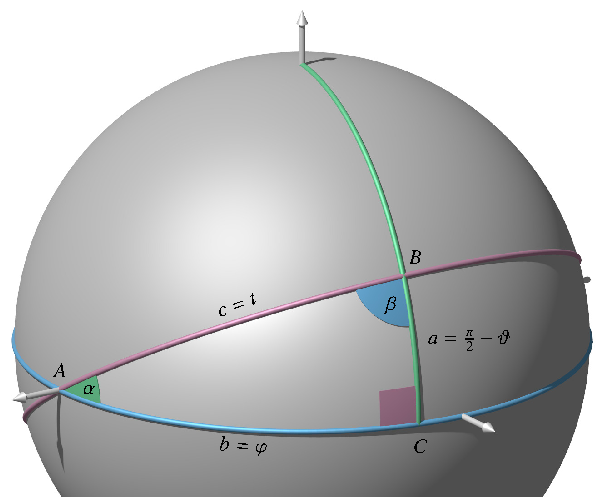
\includegraphics{chapters/100-zusammenhang/images/kugeldreieck.pdf}
\caption{Rechtwinkliges Kugeldreieck zur Parametrisierung eines
Grosskreises, der gegenüber dem Äquator um den Winkel $\alpha$ geneigt
ist.
\label{buch:zusammenhang:geodaeten:fig:kugeldreieck}}
\end{figure}
%
Damit lässt sich jetzt die Differentialgleichung für eine Geodäte auf
einer Kugel finden.
Sie ist
\begin{equation}
\left.
\begin{aligned}
\ddot{x}^1 &= -\Gamma^1_{ik}\dot{x}^i\dot{x}^k
\\
\ddot{x}^2 &= -\Gamma^2_{ik}\dot{x}^i\dot{x}^k
\end{aligned}
\quad
\right\}
\qquad\Rightarrow\qquad
\left\{
\quad
\begin{aligned}
\ddot{\vartheta}
&=
\sin\vartheta\cos\vartheta \cdot \dot{\varphi}^2
\\
\ddot{\varphi}
&=
-\cot\vartheta \cdot \dot{\vartheta}\dot{\varphi}.
\end{aligned}
\right.
\label{buch:zusammenhang:geodaeten:kugeldgl}
\end{equation}
Der Äquator ist durch $\vartheta=\frac{\pi}2$ definiert.
Für diesen Wert werden die Differentialgleichungen für $\varphi$ zu
\[
\ddot{\varphi}=0,
\]
die als Lösung eine lineare Funktion
$\varphi(0)=\omega t +\varphi_0$ hat.

Ein Längenkreis ist gegeben durch $\varphi=\text{const}$ oder
$\dot{\varphi}=0$, damit wird die Differentialgleichung für $\vartheta$
zu
\[
\ddot{\vartheta} = 0,
\]
die als Lösung eine lineare Funktion der Form
$\vartheta(t) = \omega t + \vartheta_0$ hat.

Andere Geodäten schneiden den Äquator, wir können ohne Beschränkung der
Allgemeinheit annehmen, dass dies für $\varphi=0$ geschieht.
In Abbildung~\ref{buch:zusammenhang:geodaeten:fig:kugeldreieck}
ist rot der Grosskreis durch den Punkt $A$ bei $\varphi=0$ dargestellt,
der den Äquator im Winkel $\alpha$ schneidet.
Als Parameter wird die Länge $c=t$ der Hypothenuse des rechtwinkligen
Dreiecks verwendet.
Der sphärische Sinussatz liefert die Beziehung
\[
\sin a : \sin \alpha
=
\sin c : \sin\gamma
=
\sin c,
\]
wegen $\sin\gamma=\sin\frac{\pi}2=1$.
Durch einsetzen der Werte aus der
Abbildung~\ref{buch:zusammenhang:geodaeten:fig:kugeldreieck}
erhalten wir
\begin{align*}
\sin\biggl(\frac{\pi}2-\vartheta\biggr) : \sin\alpha
&=
\sin t
\\
\cos\vartheta
&=
\sin\alpha \sin t
&&\Rightarrow&
\vartheta(t) &= \arccos(\sin\alpha\sin t).
\end{align*}
Für die Berechnung von $\varphi$ kann der sphärische Kosinussatz
für rechtwinklige sphärische Dreiecke in der Form
\begin{align*}
\cos c = \cos a\cos b
\quad\Rightarrow\quad
\cos\varphi\cos\biggl(\frac{\pi}2-\vartheta(t)\biggr)
&=
\cos t
\\
\cos\varphi
&= 
\frac{
\cos t
}{
\sin\vartheta(t)
}.
\end{align*}
Daraus erhalten wir als vollständige Parametrisierung des Grosskreises
\begin{equation}
\begin{aligned}
\vartheta(t)
&=
\arccos(\sin\alpha\cos t)
\\
\varphi(t)
&=
\arccos\frac{\cos t}{\sin\vartheta(t)}.
\end{aligned}
\label{buch:zusammenhang:geodaeten:eqn:kugelgeodaeten}
\end{equation}
Durch Nachrechnen kann geprüft werden, dass diese Funktionen tatsächlich
eine Lösung der Geodätendifferentialgleichung ergeben.
Die Rechnung ist allerdings ziemlich mühsam, die Verwendung eines
Computeralgebrasystems ist empfohlen.


%
% Geodäten als kürzeste Verbindungen
%
\subsection{Geodäten als kürzeste Verbindungen
\label{buch:zusammenhang:geodaeten:subsection:kuerzeste}}
Eine Kurve zwischen zwei Punkten kann in einer Karte durch eine Funktion
\(
t\mapsto x^i(t)
\)
beschrieben werden.
Die Länge dieser Kurve zwischen den Parameterwerten $t_A$ und $t_B$
ist durch das Integral
\begin{equation}
l
=
\int_{t_A}^{t_B}
\sqrt{g_{ik}(x) \dot{x}^i \dot{x}^k }
\,dt.
\label{buch:zusammenhang:geodaeten:eqn:funktional}
\end{equation}
Die Länge der Kurve ist nicht abhängig von der Parametrisierung, es ist
daher keine Einschränkung, ein festes Parameterintervall zu verwenden.

Die Lagrange-Funktion des Funktionals
\eqref{buch:zusammenhang:geodaeten:eqn:funktional}
ist 
\[
L(x^i, \dot{x}^i)
=
\sqrt{ g_{ik}(x) \dot{x}^i \dot{x}^k }.
\]
Die Wurzel führt dazu, dass die für die Euler-Lagrange-Differentialgleichung
nötigen partiellen Ableitungen von $L$ einen hässlichen Nenner haben.
Dies kann vermieden werden, indem die Unabhängigkeit der Weglänge von der
Parametrisierung ausgenutzt wird.
Verwendet man als Parameter die Weglänge, dann ist $L(x^i,\dot{x}^i)$
konstant.
Wir schreiben daher
\[
F(x^i,\dot{x}^i)
=
\frac12 L(x^i,\dot{x}^i)^2
\]
und verlangen von der Parametrisierung, dass 
\[
\frac{d}{dt} L(x^i, \dot{x}^i) = 0
\]
ist.
Die partiellen Ableitungen für die Euler-Lagrange-Differentialgleichungen
\begin{align*}
\frac{\partial F}{\partial x^l}
&=
L(x^i,\dot{x}^i)\, \frac{\partial L}{\partial x^l} (x^i,\dot{x}^i)
\\
\frac{\partial F}{\partial \dot{x}^l}
&=
L(x^i,\dot{x}^i)\, \frac{\partial L}{\partial \dot{x}^l} (x^i,\dot{x}^i).
\end{align*}
Damit wird die Euler-Lagrange-Differentialgleichung für $F$ zu
\begin{align*}
\frac{\partial F}{\partial x^l}
-
\frac{d}{dt}\frac{\partial F}{\partial \dot{x}^l}
&=
L
\frac{\partial L}{\partial x^l}
-
\frac{d}{dt}\biggl(
L
\frac{\partial L}{\partial\dot{x}^l}
\biggr)
\\
&=
L(x^i,\dot{x}^i)
\frac{\partial L}{\partial x^l}
-
\frac{dL}{dt}
\frac{\partial L}{\partial\dot{x}^l}
-
L
\frac{d}{dt}
\frac{\partial L}{\partial\dot{x}^l}.
\intertext{Da $L$ konstant ist, fällt der mittlere Term weg und es
bleibt}
\frac{\partial F}{\partial x^l}
-
\frac{d}{dt}\frac{\partial F}{\partial \dot{x}^l}
&=
L
\cdot
\biggl(
\frac{\partial L}{\partial x^l}
-
\frac{d}{dt}
\frac{\partial L}{\partial\dot{x}^l}
\biggr).
\end{align*}
Da $L$ konstant und verschieden von $0$ ist, verschwindet die rechte
Seite nur dann, wenn auch die linke Seite verschwindet.
Statt der Lagrange-Funktion $L(x^i,\dot{x}^i)$ kann also mit gleichem
Resultat die Lagrange-Funktion $f(x^i,\dot{x}^i)$ verwendet
werden.

Die partiellen Ableitungen der Lagrange-Funktion sind
\begin{align*}
\frac{\partial F}{\partial x^l}
&=
\frac12
\frac{\partial g_{ik}}{\partial x^l}
\dot{x}^i\dot{x}^k
\\
\frac{\partial F}{\partial \dot{x}^l}
&=
\frac12
g_{ik}(\dot{x}^i\delta_i^l\dot{x}^k + \dot{x}^i\dot{x}^k\delta_k^l)
=
\frac12
\bigl(
g_{lk}\dot{x}^k
+
g_{il}\dot{x}^i
\bigr).
\intertext{Für die Euler-Lagrange-Differentialgleichung ist jetzt auch
noch die Ableitung nach $t$ zu bestimmen:}
\frac{d}{dt}
\frac{\partial F}{\partial x^l}
&=
\frac12
\biggl(
\frac{\partial g_{lk}}{\partial x^s}\dot{x}^s\dot{x}^k
+
g_{lk}\ddot{x}^k
+
\frac{\partial g_{il}}{\partial x^s}\dot{x}^s\dot{x}^i
+
g_{il}\ddot{x}^i
\biggr).
\end{align*}
Damit wird die Euler-Lagrange-Differentialgleichung
\begin{align*}
0
&=
\frac{\partial F}{\partial x^l}
-
\frac{d}{dt}\frac{\partial F}{\partial\dot{x}^l}
\\
&=
\frac12
\biggl(
\frac{\partial g_{ik}}{\partial x^l}
\dot{x}^i\dot{x}^k
-
\frac{\partial g_{lk}}{\partial x^s}\dot{x}^s\dot{x}^k
-
\frac{\partial g_{il}}{\partial x^s}\dot{x}^s\dot{x}^i
\biggr)
-
\frac12
g_{lk}\ddot{x}^k
-
\frac12
g_{lk}\ddot{x}^k
\\
&=
\frac12
\biggl(
\frac{\partial g_{ik}}{\partial x^l}
\dot{x}^i\dot{x}^k
-
\frac{\partial g_{lk}}{\partial x^i}\dot{x}^i\dot{x}^k
-
\frac{\partial g_{il}}{\partial x^k}\dot{x}^k\dot{x}^i
\biggr)
-
g_{lk}\ddot{x}^k
\\
&=
\frac12
\biggl(
\frac{\partial g_{ik}}{\partial x^l}
-
\frac{\partial g_{lk}}{\partial x^i}
-
\frac{\partial g_{il}}{\partial x^k}
\biggr)
\dot{x}^i\dot{x}^k
-
g_{lk}\ddot{x}^k
\\
&=
-\Gamma_{l,ik} \dot{x}^i\dot{x}^k
-
g_{lk} \ddot{x}^k.
\end{align*}
Multipliziert man dies mit den Einträgen $g^{jl}$ der inversen
Matrix von $g$ und summiert über $l$, ergibt sich
\[
0
=
g^{jl}\Gamma_{l,ik}\dot{x}^i\dot{x}^k+g^{jl}g_{lk}\ddot{x}^k
=
\Gamma^j_{ik}\dot{x}^i\dot{x}^k + \delta^j_k\ddot{x}^k
=
\Gamma^j_{ik}\dot{x}^i\dot{x}^k + \ddot{x}^j.
\]
Die Euler-Lagrange-Differentialgleichung für das Weglängenfunktional
ist also die Differentialgleichung für Geodäten.

%
% Die Exponentialabbildung
%
\subsection{Die Exponentialabbildung
\label{buch:zusammenhang:subsection:exponentialabbildung}}
Sei jetzt $p\in M$ ein Punkt einer $n$-dimensionalen riemannschen
Mannigfaltigkeit und $\vec{v}\in T_pM$ ein Tangentialvektor in $p$.
Die Differentialgleichung der Geodäten garantiert, dass es mindestens
in einer Umgebung von $0\subset\mathbb{R}$ eine Lösungskurve
$\gamma(t)$ gibt mit $\gamma(0)=p$ und $\dot{\gamma}(t)=\vec{v}$.

\begin{definition}[Exponentialabbildung]
\label{buch:zusammenhang:geodaeten:def:exponentialabbildung}
Die \emph{Exponentialabbildung} im Punkt $p$ einer riemannschen
\index{Exponentialabbildung}%
Mannigfaltigkeit $M$ ist diejenige Abbildung einer Umgebung $U\subset T_pM$
nach $M$ mit der Eigenschaft, dass $\exp_p(t\vec{v})$ eine Geodäte
durch $p$ mit Tangentialvektor
\[
\frac{d}{dt}
\exp_p(t\vec{v})\bigg|_{t=0}
=
\vec{v}
\]
ist.
\end{definition}

Gleichbedeutend mit der
Definition~\ref{buch:zusammenhang:geodaeten:def:exponentialabbildung}
ist die folgende Konstruktion.
Um das Bild $\exp_p(\vec{v})$ zu finden, konstruiert man die
Geodäte $\gamma(t)$ durch $p$ mit Richtungsvektor $\dot{\gamma}(0)=\vec{v}$.
Dann ist $\exp_p(\vec{v})=\gamma(1)$.
Diese Definition verlangt aber, dass die Kurve $\gamma(t)$ auch tatsächlich
für beliebige Zeit $t$ definiert ist.
Die üblichen Sätze über gewöhnliche Differentialgleichungen wie der
Satz von Picard-Lindelöf garantieren die Existenz einer Lösung nur
\index{Satz von Picard-Lindelöf}%
für eine offene Umgebung von $t=0$.

Der Satz von Picard-Lindelöf gilt für eine Differentialgleichung
in der Form $\dot{x} = f(t,x)$ mit einer Funktion
$f\colon\mathbb{R}\times\mathbb{R}^n \to \mathbb{R}^n$, die im zweiten
Argument eine Lipschitz-Bedingung erfüllt.
\index{Lipschitz-Bedingung}%
Diese garantiert, dass die Ableitung $\dot{x}$ nicht zu gross wird und
damit die Lösung $x(t)$ divergiert.
Es ist wohlbekannt, dass für stärkere Bedingungen an die die Funktion $f$ 
die Lösung für beliebige Zeit $t$ existiert.
Zum Beispiel ist die Lösung der linearen Differentialgleichung
$\dot{x}=Ax$ mit einer Matrix $A\in M_{n\times n}(\mathbb{R})$
durch die Matrixexponentialfunktion $x(t) = e^{At}x_0$ gegeben, die
für beliebige $t\in\mathbb{R}$ definiert ist.
Sogar wenn die Matrix $A$ in einem Intervall $I\subset\mathbb{R}$
auf glatte Art von $t$ abhängt lässt sich zeigen, dass sich eine
Lösung immer auf das ganze Intervall ausdehnen lässt.
Ein Beweis wird in \cite[Theorem 4.31]{buch:leerm} gegeben.

Die Differentialgleichung der Geodäten erfüllt aber eine noch 
stärkere Bedingung.
Entlang einer Lösung wird der Tangentialvektor $\dot{\gamma}(t)$ 
für alle Zeiten, für die die Lösung definiert ist, parallel transportiert.
Insbesondere bleibt seine Länge immer gleich gross, es besteht gar
nicht die Gefahr, dass $\dot{\gamma}(t)$ divergiert.
Was hingegen geschehen könnte ist, dass $\gamma(t)$ in $M$ nicht
mehr definiert werden kann.

Es gibt natürlich Fälle, wo es unvermeidlich ist, dass $\gamma(t)$
nur für ein Intervall $(a,b)$ definiert sein kann.
In einer beschränkten offenen Menge in $\mathbb{R}^n$ sind die Geodäten
Geraden.
Sie sind nur solange definiert, als $\gamma(t)$ die Menge
nicht verlässt.
Auf einer kompakten Mannigfaltigkeit ohne Rand kann dies nicht passieren,
dort dürfen wir annehmen, dass der Grenzwert $\gamma(t)$ für $t\to b$
wieder in $M$ liegt.
Das Argument zeigt also, dass eine Geodäte nicht irgendwo im inneren
einer riemannschen Mannigfaltigkeit enden kann.
Wenn der Grenzwert $\gamma(t)$ für $t\to b$ in $M$ existiert, dann
lässt sich die Geodäte auch darüber hinaus fortsetzen.

Wenn sich die Geodäte auf beliebige Parameter $t\in\mathbb{R}$
ausdehen lässt, nennen wir die Mannigfaltigkeit geodätisch vollständig.
Als formale Definition verwenden wir die folgende.

\begin{definition}[geodätisch vollständig]
\label{buch:zusammenhang:geodaeten:def:vollst}
Eine riemannsche Mannigfaltigkeit $M$ heisst \emph{geodätisch vollständig},
wenn die Exponentialabbildung $\exp_p$ für jeden Punkt $p\in M$
auf ganz $T_pM$ definiert ist.
\index{geodätisch vollständig}%
\end{definition}

In vielen Fällen ist die Voraussetzung der geodätischen Vollständigkeit
nicht nötig.
Die allgemeine Relativitätstheorie beschreibt zum Beispiel die Bahnen
von Teilchen oder Lichtstrahlen als Geodäten in einer pseudoriemannschen
Mannigfaltigkeit.
\index{Universum}%
Wir wissen nicht, ob das Universum geodätisch vollständig ist im
mathematischen Sinn der
Definition~\ref{buch:zusammenhang:geodaeten:def:vollst}.
Wir dürfen aber davon ausgehen, dass die Exponentialabbildung für alle
praktisch sinnvollen Tangentialvektoren definiert ist.

Die Definition der Exponentialabbildung verlangt, dass man entlang einer
Geodäten vom Ausgangspunkt $p$ zum Endpunkt $\exp_p(\vec{v})$ gelangen
kann.
Der Definitionsbereich der Exponentialabbildung muss also die Eigenschaft
haben, dass mit jedem Vektor $\vec{v}$ auch die Strecke zwischen dem Nullpunkt
und $\vec{v}$ im Definitionsbereich enthalten ist.
Solche Mengen heissen \emph{sternförmig}.

\begin{definition}[sternförmig]
\label{buch:zusammenhang:geodaeten:def:sternfoermig}
Eine Teilmenge $U\subset V$ eines Vektorraumes heisst \emph{sternförmig},
wenn mit jedem Punkt $u\in U$ auch alle skalierten Vektoren $tu\in U$
mit $t\in [0,1]$ in $U$ sind.
\index{sternformig@sternförmig}%
\end{definition}

%
% Normalkoordinaten
%
\subsection{Normalkoordinaten}
Die Exponentialabbildung kann dazu verwendet werden, in der
Umgebung eines Punktes der Mannigfaltigkeit ein Koordinatensystem
zu definieren, in dem die Christoffel-Symbole besonders einfache
Form annehmen.

\begin{definition}[Normale Umgebung]
Eine \emph{normale Umgebung} eines Punktes $p$ in einer 
riemannschen Mannigfaltigkeit ist eine offene Menge $U\subset M$,
die diffeomorphes Bild einer sternförmigen Menge in $T_pM$ ist.
\end{definition}

In einer normalen Umgebung kann man jetzt Koordinaten einführen,
indem man in $T_pM$ eine Basis wählt.
Bilden die Vektoren $b_1,\dots,b_n$ eine Basis, dann gibt es reelle
Zahlen $v^1,\dots,v^n$ mit 
\[
\exp_p(v^1b_1+\dots+v^nb_n)=u.
\]
Diese Abbildung ist die Zusammensetzung der 
Abbildung
\[
B
\colon
\mathbb{R}^n \to T_pM
:
(v^1,\dots,v^n)
\mapsto
v^1b_1+\dots+v^nb_n
\]
mit der Exponentialabbildung.
Sie ist definiert, solange $B\xi$ im Definitionsbereich von $\exp_p$
enthalten ist.
Die Umkehrung $B^{-1}\circ\exp_p^{-1}$ ist eine Karte auf $U$.

Wählt man für $b_1,\dots,b_n$ eine orthonormale Basis von $T_pM$,
dann entsteht eine Karte mit sogenannten \emph{Normalkoordinaten}
zentriert im Punkt $p$,
die sich durch besondere Eigenschaften auszeichnen.
Zunächst sind nach Konstruktion die zur Basis gehörigen Tangentialvektoren
orthonormiert, so dass der metrische Tensor durch $g_{ik}=\delta_{ik}$
gegeben ist.

\begin{satz}[Eigenschaften von Normalkoordinaten]
\label{zusammenhang:geodaeten:satz:normalkoordinaten}
Sei $M$ eine $n$-dimensionale riemannsche Mannigfaltigkeit und $(U,x^i)$
ein Normalkoordinatensystem im Punkt $p\in M$.
Dann gilt
\begin{enumerate}
\item Die Koordinaten von $p$  sind $(0,\dots,0)$.
\item Die Komponenten des metrischen Tensors in $p$ sind $g_{ik}=\delta_{ik}$.
\item Für jeden Tangentialvektor $v=v^i\partial_i$ ist die Geodäte mit
Richtung $v$ in Normalkoordinaten gegeben durch $(tv^1,\dots,tv^n)$.
\item Die Christoffelsymbole $\Gamma^i_{kl}$ verschwinden im Punkt $p$.
\item Alle ersten partiellen Ableitungen der metrischen Koeffizienten
verschwinden im Punkt $p$.
\item Die ersten partiellen Ableitungen von $g^{ik}$ verschwinden im Punkt $p$.
\end{enumerate}
\end{satz}

\begin{proof}
Die ersten drei Eigenshaften ergeben sich unmittelbar aus der Definition
der Normalkoordinaten.
Da die Geodäten Geraden sind, verschwinden die zweiten Ableitungen
der Koordinaten eines Geodätenpunkts.
Die Geodätengleichungen reduzieren sich damit auf
\[
\Gamma^i_{kl} v^kv^l = 0
\]
im Punkt $p$.
Durch Einsetzen der Basisvektoren $b_a$ mit Koordinaten $\delta_a^i$
bekommt man daraus zunächst
\begin{equation}
0
=
\Gamma^i_{kl}v^kv^l
=
\Gamma^i_{kl}\delta_a^k\delta_a^l
=
\Gamma^i_{aa}.
\label{buch:zusammenhang:geodaeten:eqn:Giaa}
\end{equation}
Setzt man Linearkombinationen $b_a\pm b_b$ mit den Koordinaten
$\delta_a^i\pm \delta_b^i$ für $v$ ein, erhält man
\begin{align*}
0
&=
\Gamma^i_{kl} (\delta_a^k \pm \delta_b^k)(\delta_a^l \pm \delta_b^l)
\\
&=
\Gamma^i_{kl}(
    \delta_a^k\delta_a^l
\pm \delta_a^k\delta_b^l
\pm \delta_b^k\delta_a^l
  + \delta_b^k\delta_b^l
)
\\
&=
\Gamma^i_{aa}
\pm
\Gamma^i_{ab}
\pm
\Gamma^i_{ba}
+
\Gamma^i_{bb}
\\
&=
\pm
2
\Gamma^i_{ab},
\end{align*}
wobei sowohl
\eqref{buch:zusammenhang:geodaeten:eqn:Giaa}
als auch die Symmetrie der Christoffelsymbole verwendet wurden.

Die Christoffelsymbole des Levi-Cività-Zusammenhangs ergaben sich
als Lösungen des Gleichungssystems~\ref{buch:zusammenhang:kovabl:eqn:gGamma}.
Im Punkt $p$ vereinfachen Sie sich wegen $g_{ik}=\delta_{ik}$ zu
\[
\frac{\partial g_{il}}{\partial x_k}
=
g_{sl}\Gamma^s_{ik}
+
g_{is}\Gamma^s_{lk}
=
\delta_{sl}\Gamma^s_{ik}
+
\delta_{is}\Gamma^s_{lk}
=
\Gamma^l_{ik}
+
\Gamma^i_{lk}
=
0,
\]
da die Christoffelsymbole verschwinden.

Auch die Ableitungen von $g^{ik}$ verschwinden im Punkt $0$.
Dies lässt sich noch viel allgemeiner beweisen.
Seien $A(t)$ und $B(t)$ inverse Matrizen mit $A(0)=B(0)=I$, die von einem
Parameter $t$ abhängen.
Ausserdem sei $\dot{A}(0)=0$
Dann ist die Ableitung des Produktes $A(t)B(t)=I$
\begin{align*}
\frac{d}{dt}I\bigg|_{t=0}
&=
\biggl(
\frac{dA}{dt}(t) B(t)
+
A(t)
\frac{dB}{dt}(t)
\biggr)\bigg|_{t=0}
\\
&=
\dot{A}(0)
B(0)
+
A(0)
\dot{B}(0)
=
\dot{A}(0)
+
\dot{B}(0)
=
\dot{B}(0).
\end{align*}
Somit verschwindet auch die erste Ableitung der inversen Matrix von $A$.
Angewendet auf $A=g_{ik}$ und $B=g^{ik}$ und eine der Koordinaten als
Parameter folgt, dass die partiellen ersten Ableitungen von $g^{ik}$
an der Stelle $p$ ebenfalls verschwinden.
\end{proof}

Die speziell einfache Form der Christoffelsymbole in Normalkoordinaten
wird später ermöglichen, auch den riemannschen Krümmungstensor an der
Stelle zu berechnen.

%
% Kovariante Ableitung in Normalkoordinaten
%
\subsubsection{Kovariante Ableitung in Normalkoordinaten}
In Normalkoordinaten verschwinden die Christoffelsymbole im Punkt $p$.
Dies macht die Berechnung der kovarianten Ableitung besonders einfach.
Ist $A$ in kontravarianter Tensor mit den Komponenten $A_i$, dann ist
die kovariante Ableitung in Richtung des Vektors $V$ mit den Komponenten
$v^i$ an der Stelle $p$
\begin{align}
\nabla_X A
&=
\biggl(
\frac{\partial A^i}{\partial x^k}
+
\Gamma^i_{kl} A^l
\biggr)
v^k
\frac{\partial}{\partial x^i}
=
\frac{\partial A^i}{\partial x^k}
v^k
\frac{\partial}{\partial x^i}
&&\text{oder}
&
A^i_{;k}
&=
\frac{\partial A^i}{\partial x^k}
.
\label{buch:zusammenhang:geodaeten:eqn:kovablnormalkontravariant}
\intertext{Für einen kovarianten Tensor $B$ mit Komponenten $B_i$ wird
die kovariante Ableitung
nach Definition~\ref{buch:zusammenhang:parallel:definition:kovabl1form}
zu}
\nabla_X B
&=
\biggl(
\frac{\partial B_i}{\partial x^k}
-
\Gamma^l_{ik} B_l
\biggr)
v^k
\,dx^i
=
\frac{\partial B_i}{\partial x^k}
v^k
\,dx^i
&&\text{oder}
&
B_{i;k}
&=
\frac{\partial B_i}{\partial x^k}
\label{buch:zusammenhang:geodaeten:eqn:kovablnormalkovariant}
\end{align}
In Normalkoordinaten an der Stelle $p$ fällt die kovariante Ableitung
mit der Richtungsableitung zusammen.




